% Generated by thesis/ch7/exp1/c4_units_figures.py -- do not edit by hand.
\begin{figure}[p]
  \centering
  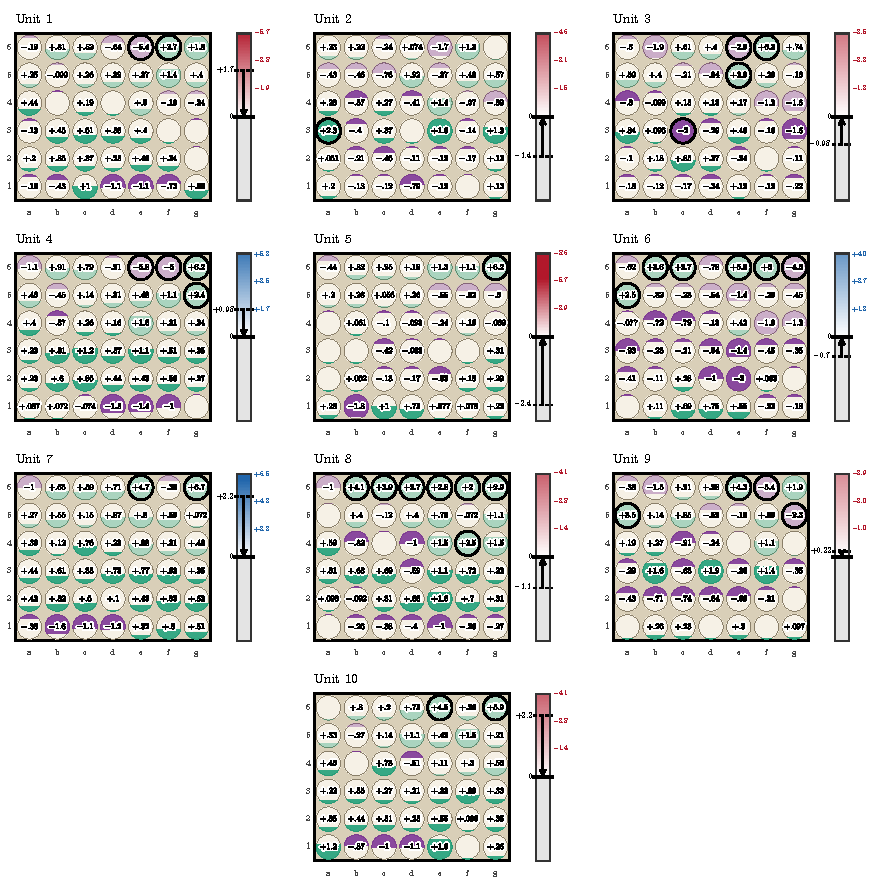
\includegraphics[width=\textwidth,height=0.9\textheight,keepaspectratio]{figures/ch7/c4-units-all.pdf}
  \caption{Connect-4 cells network: each hidden unit as a board. Number in each hole: points per piece (the change in the unit's level when the square holds an x; an o gives the opposite). Green filling from the bottom: an x there pushes the unit towards firing; purple from the top: away; full hole: 2 points or more; ring: more than 2; pale: filled in under 5\% of positions. Bar: the unit's level; it fires above the thick line (level 0) and is silent below it (grey); dashed line and arrow: the level on an empty board and the gap pieces must close; ticks and shading on the right: the change in x's log-odds at levels 1, 2 and 3 (blue helps x, red hurts x).}
  \label{fig:ch7-c4-units-all}
\end{figure}
